\section {Present de la IA}
Actualment, el camp de la IA s'ha especialitzat molt: \emph{aprenentatge de màquina}, \emph{robòtica aplicada}, \emph{deducció, raonament i solució de problemes}, \emph{processament de llenguatge natural}, \emph{moció i manipulació}, \emph{percepció}, \emph{intel·ligència social}, \emph{creativitat}, i l'objectiu final: \emph{intel·ligència artificial general}, que combina tots els aspectes.

En el nostre dia a dia i han molts programes que utilitzen intel·ligència artificial (de forma més o menys proficient) sense que ens n'adonem, com per exemple, el \emph{traductor de Google}: sembla molt fàcil buscar al diccionari les paraules que es demanen per a traduir, però una traducció literal mai és satisfactòria, per això es segueixen procediments intel·ligents que permeten realitzar traduccions naturals.

\emph{YouTube} i \emph{Google} utilitzen algorismes intel·ligents per a filtrar resultats de cerca segons els teus gustos. \emph{eBay} i \emph{Amazon} també ho fan, recomanant productes d'acord amb el teu historial de compra.


Pel que fa l'àmbit de la robòtica, s'han creat robots capaços de caminar de forma òptima i evitar caigudes causades per els diferents tipus de terreny intentant simular animals com
ara gossos en córrer. També s'han creat humanoides, robots amb forma de persones, que són capaços de fer moviments humans, per exemple abraçar expressar emocions i manipular certs objectes. \cite{bostondynamics}


Un altre exemple d'intel·ligència artificial és la que s'utilitza per complementar (o formar) un programa informàtic; el reconeixement per veu es un bon exemple. \emph{Apple} utilitza la interpretació de la veu humana per a crear una aplicació que respon a qualsevol pregunta.

\section {Futur de la IA}
És difícil predir quin serà el futur de la intel·ligència artificial, però podem establir uns objectius per al futur.

Un dels objectius que tenen la majoria de persones que treballen en la IA és aconseguir que aquesta intel·ligència deixi de ser tant especifica i passi a ser global; capaç d'aprendre
qualsevol cosa, analitzar-la de manera intel·ligent i pensar bàsicament com les persones humanes. Aquest objectiu encara és difícil d'aconseguir perquè si volem que pensin com a éssers
humans primer hem de saber perquè pensem com a éssers humans.

Aquest concepte pot semblar estrany però el que pretenem dir és que hem d'entendre primer com funciona el nostre cervell
per raonar, com reacciona en situacions que no coneix i com emmagatzema informació. Per tant podem dir que la IA pot estar lligada a la neurociència i que, en part,
depèn d'ella; el desenvolupament de la neurociència porta de la ma el desenvolupament de la intel·ligència artificial.


Un altre dels objectius de futur de la IA és el que fa referència a la intel·ligència específica, i en aquest cas està més a l'abast dels programadors. Un dels molts projectes de aquesta
intel·ligència és el de cotxes que siguin capaços de conduir sense la necessitat de un conductor. Aquest programa podria evitar molts accidents causats pel consum de drogues o
d'alcohol, i la incapacitat de persones grans al volant, fent més segures les carreteres i evitant errors humans que a qualsevol persona podem passar-li.

%\section {Perillositat de la IA}
%La discussió de si pot arribar a ser perillosa o no una IA capaç %de pensar com un humà dóna molt a parlar i discutir ja que s'han %de tenir en compte molts factors.

%Si en algun moment s'aconsegueix una intel·ligència artificial capaç de pensar com els humans però de una manera més eficient i calculadora, si tingués ment per pensar i raonar podria arribar
%a pensar que nosaltres, els éssers humans, no tenim cap funció ja que faríem el mateix que fan elles però de una manera menys eficient amb més defectes i això la podria fer pensar que hauríem
%de desaparèixer i per tant ella voldria eliminar als seus creadors. No seria perquè ens tingués odi, però tampoc ens tindria amor ni compassió, simplement pensaria que som inservibles i per tant
%ens eliminaria com si nosaltres tiréssim una joguina o un electrodomèstic a la paperera perquè ja l'únic que fa es ocupar-nos espai que podria ser utilitzat per una altre cosa, i pel que fa
%els éssers humans estaríem gastant recursos que podrien ser utilitzats per recerca. Aquesta situació espantosa i clarament alarmant es podria evitar aplicant un dels dos factors més importants
%que fan els ésser humans tal com són: els valors i les emocions. Si ens preguntessin que ens diferencia del animals diríem que clarament és la intel·ligència, que en part és veritat, però el
%factors que ens permet viure en comunitat i diferenciar-nos dels animals són els valors, que ens impedeixen fer accions que estan en contra la nostra moral, i les emocions, que ens permeten
%reaccionar amb l'exterior. Per tant si una màquina té valors i emocions i nosaltres la tractem com un igual no tindria el pensament de eliminar-nos i podria viure ajudant-nos màquines i humans.

\section {Velocitat d'evolució}
Es podria dir que hem avançat molt en el camp de la intel·ligència artificial en els últims anys, però tenim problemes per a continuar evolucionant. Això és
donat per diversos factors \cite{pbs}:
\begin {itemize}
\item \emph{Neurociència:} com hem explicat en un dels apartats anteriors, encara es té un desconeixement molt gran sobre el funcionament del cervell; això impedeix simular-lo, evidentment.
\item \emph{Desconeixent general:} hi ha un clar desconeixement general de la intel·ligència artificial, degut a que es tracta d'un camp en continuu desenvolupament, amb molts poques \emph{lleis} que es segueixen al peu de la lletra en qualsevol cas, i molts models matemàtics que materialitzar.
\item \emph{Falta d'inversió:} els governs d'avui en dia no consideren un factor important la intel·ligència artificial i aquest factor va lligat amb el factor anterior: el desconeixement.
\item \emph{Poder computacional:} si en una cosa coincideixen molts científics, es en que el cervell és una màquina de càlcul molt potent, que realitza interconnexions de forma molt ràpida, continua, i paral·lela. Els ordinadors han d'avançar en poder computacional per a poder establir-se al nivell del cervell humà, o s'han d'optimitzar els algorismes. Tot i la increïble potència dels processadors actuals (\emph{1,16 bilions} de transistors en un de quatre nuclis), s'estima que el cervell té \emph{100 bilions} de neurones. A més a més, un transistor no es tradueix a una neurona, la qual cosa implica multiplicar el nombre final per arribar a una quantitat de transistors realista.
\end {itemize}

\begin{figure}[ht!]
\centering
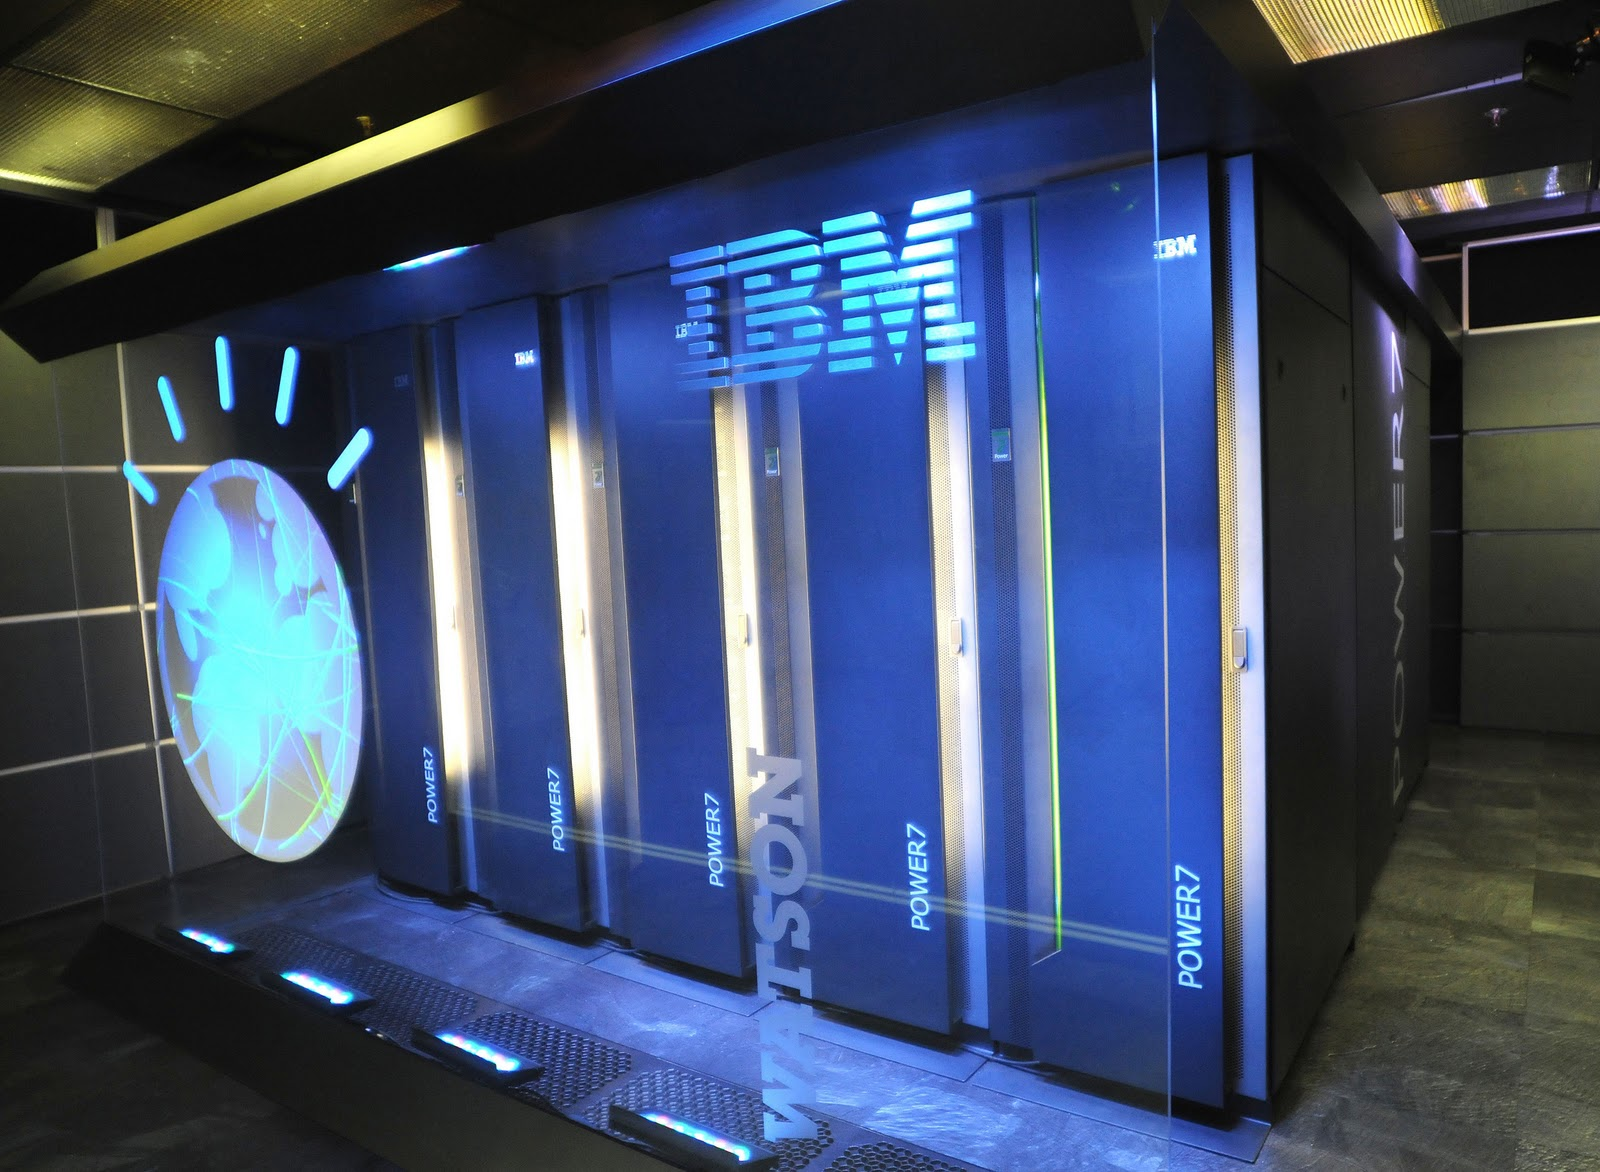
\includegraphics[height=75mm]{data/watson.jpg}
\caption{El \emph{super-ordinador} d'IBM, \emph{Watson}, posseeix 16,000 gigabytes de memòria RAM (comparats amb els 4 d'un ordinador corrent), 90 processadors de 8 nuclis cadascun (720 nuclis en total, comparats amb els 2 d'un ordinador corrent), i 4,000 gigabytes de disc dur (comparats amb els 500 d'un ordinador corrent) \cite{watsonspecs}. Va guanyar als dos millors oponents del programa nord-americà \emph{Jeopardy!} \cite{watsonjeopardy}.}
\label{watson}
\end{figure}
